\documentclass[11pt]{extarticle}
\usepackage{unicode-math}
\usepackage{mathrsfs}
\usepackage{amsthm,graphicx,xcolor,natbib,enumitem,booktabs,tabularx}
\usepackage[paperwidth=126mm, paperheight=96mm, top=5mm, bottom=5mm, right=5mm, left=5mm]{geometry}
\pagenumbering{gobble}

\usepackage[BoldFont,SlantFont]{xeCJK}  
\xeCJKsetemboldenfactor{2}
\setCJKmainfont{cwTeX Q Yuan Medium}

\usepackage{hyperref}
\hypersetup{
  colorlinks,
  linkcolor={red!50!black},
  citecolor={blue!60!black},
  urlcolor={blue!60!black}
}

\newcommand{\ds}{\displaystyle}
\newcommand{\ie}{\;\Longrightarrow\;}
\newcommand{\ifff}{\;\Longleftrightarrow\;}
\newcommand{\mi}{\mathrm{i}}
\DeclareMathOperator*{\dom}{dom}
\DeclareMathOperator*{\codom}{codom}
\DeclareMathOperator*{\ran}{ran}
\newcommand{\floor}[1]{\lfloor #1 \rfloor}
\newcommand{\ceil}[1]{\lceil #1 \rceil}
\newcommand{\Set}[2]{\big\{ \ #1\ \big|\ #2\ \big\}}
\newcommand{\pdiff}[2]{\frac{\partial\hfil#1\hfil}{\partial #2}}
\newcommand{\vx}{\symbfup{x}}
\newcommand{\vw}{\symbfup{w}}
\newcommand{\vb}{\symbfup{b}}

\DeclareMathOperator\prb{{\sf P}}
\DeclareMathOperator\expc{{\sf E}}
\DeclareMathOperator\var{var}
\DeclareMathOperator\cov{cov}
\DeclareMathOperator\cor{cor}
\DeclareMathOperator*{\argmax}{\arg\!\max}
\DeclareMathOperator*{\argmin}{\arg\!\min}
\DeclareMathOperator*{\im}{Im}
\DeclareMathOperator*{\re}{Re}
\DeclareMathOperator*{\conv}{conv}
\DeclareMathOperator*{\proj}{proj}
\DeclareMathOperator*{\tr}{tr}
\DeclareMathOperator*{\diag}{diag}
\DeclareMathOperator*{\epi}{epi}
\DeclareMathOperator*{\dist}{dist}
\DeclareMathOperator*{\inte}{int}
\DeclareMathOperator*{\relint}{relint}

\theoremstyle{definition}
\newtheorem*{dfn}{Definition}
\newtheorem*{prp}{Property}
\newtheorem*{thm}{Theorem}
\newtheorem*{ex}{Example}
\newtheorem*{sol}{Solution}
\newtheorem*{prf}{Proof}

\newcommand\scalemath[2]{\scalebox{#1}{\mbox{\ensuremath{\displaystyle #2}}}}

\begin{document}
\title{\texorpdfstring{\vspace{15mm} Operations Research\\ 09. Support Vector Machine (SVM)}{Operations Research\\ 09. Support Vector Machine (SVM)}} 
\author{}
\date{}
\maketitle

\newpage

\section*{Binary Classification}

Given the data $\ds\{(\vx_i, y_i)\}_{i=1}^m$, $\ds y_i\in\{-1, +1\}$, $\ds\vx_i\in\mathbb{R}^n$, find the hyperplane with maximum ``margin'' --- the gap between parallel hyperplanes seperating two classes where the vectors of neither class can lie

\vspace{-5mm}
\begin{figure}[!htbp]
  \centering
  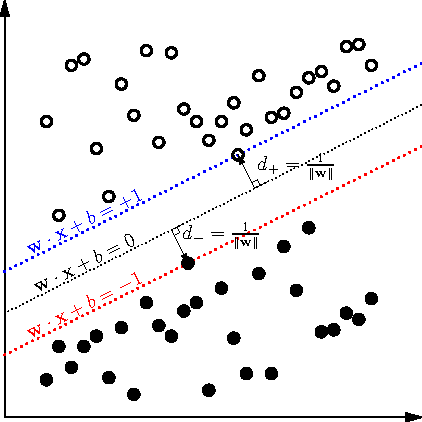
\includegraphics[scale=0.8]{fig/d1.pdf}
\end{figure}

\newpage

\section*{SVM: Linearly Separable (Hard-Margin)}

\noindent Let $\vw\cdot\vx + b=0$ be the seperating hyperplane and $d_+, d_-$ be the shortest distance to the closest objects from the class $+1$, $-1$, respectively.

\bigskip\bigskip
\noindent Suppose that
\begin{align*}
  \vw\cdot\vx_i + b &\geqslant +1 \quad\text{ for }\,y_i = +1\\
  \vw\cdot\vx_i + b &\leqslant -1 \quad\text{ for }\,y_i = -1
\end{align*}
which can be combined as
\begin{align*}
  1 - y_i\left(\vw\cdot\vx_i + b \right)\leqslant 0,\quad\forall\,i = 1,\,2,\,\ldots,\,m
\end{align*}

\bigskip
\begin{thm}
  The distance between planes $\ds\vw\cdot\vx = b_1$ and $\vw\cdot\vx = b_2$ is $\ds\frac{|b_1 - b_2|}{\|\vw\|}$. 
\end{thm}

\begin{prf}
  For $\vx_1$, $\vx_2$ s.t. $\ds\vw\cdot\vx_1 = b_1$, $\ds\vw\cdot\vx_2 = b_2$ and $\overline{\vx_1 \vx_2}$ be the shortest path, $\ds\exists\,t\in\mathbb{R}$ such that $\ds \vx_1 - \vx_2 = t\,\vw\ie b_1 - b_2 = \vw\cdot(\vx_1 - \vx_2) = t\,\vw\cdot\vw = t\,\|\vw\|^2 \ie t = \frac{b_1 - b_2}{\|\vw\|^2}$. So the distance is $\ds\|t\,\vw\| = \frac{|b_1 - b_2|}{\|\vw\|}$.
\end{prf}

\bigskip
\noindent The margin between $\ds\vw\cdot\vx = 1 - b$ and $\ds\vw\cdot\vx = -1 - b$ is simply $\ds\frac{2}{\|\vw\|}$.
  %\item Let $\vx_0$ be a point on $\vw\cdot\vx + b = 0$, then $\vx_0$ projected on $\vw\cdot\vx + b = 1$ is $\vx_0 + t\,\vw$ with $t$ to be determined; we have
  %  \begin{align*}
  %    \vw\cdot\left(\vx_0 + t\vw\right) + \vb = 1\ie t = \frac{1}{\|\vw\|^2}\ie d_+ = \|t\,\vw\| = \frac{1}{\|\vw\|}
  %  \end{align*}
  %\item By the same token, $\ds d_- = \frac{1}{\|\vw\|}$; the margin $\ds=d_+ + d_-=\frac{2}{\|\vw\|}$.

\bigskip\bigskip
\noindent Determine the hyperplane with maximum margin
\begin{align*}
  &\text{maximize }\frac{1}{\|\vw\|}\ifff\text{minimize }\frac{1}{2}\,\|\vw\|^2 \\
  &\text{subject to}\quad 1 - y_i\left(\vw\cdot\vx_i + b \right)\leqslant 0\quad\forall\,i = 1,\,2,\,\ldots,\,m.
\end{align*}

\bigskip
\noindent Set the Lagrangian $\mathcal{L}$
\begin{align}\label{f:lag}
  \mathcal{L} = \frac{1}{2}\|\vw\|^2 + \sum_{i=1}^m\lambda_i\left\{1 - y_i\left(\vw\cdot\vx_i + b\right)\right\}
\end{align}

\newpage

\noindent The KKT conditions are
\begin{equation}
\begin{aligned}\label{f:kkt}
  &\frac{\partial\mathcal{L}}{\partial \vw} = 0 \ie \vw=\sum_{i=1}^m\lambda_i\,y_i\,\vx_i\\
  &\frac{\partial\mathcal{L}}{\partial b} = 0 \ie \sum_{i=1}^m\lambda_i\,y_i=0\\
  & 1- y_i\left(\vw\cdot\vx_i + b \right) \leqslant 0,\quad i=1,\,2,\,\ldots,\,m\\
  &\lambda_i\geqslant 0,\quad i=1,\,2,\,\ldots,\,m\\
  &\lambda_i\left\{1 - y_i\left(\vw\cdot\vx_i + b \right)\right\}=0,\quad i=1,\,2,\,\ldots,\,m
\end{aligned}
\end{equation}
Substitute the KKT conditions (\ref{f:kkt}) into $\mathcal{L}$ (\ref{f:lag}), the dual Lagrangian
\begin{align*}
  \mathcal{L}_D=\sum_{i=1}^m\lambda_i-\frac{1}{2}\sum_{i=1}^m\sum_{j=1}^m\lambda_i\lambda_j\,y_i\,y_j\,\vx_i^\top\vx_j
\end{align*}
Now the problem becomes maximizing $\mathcal{L}_D$ subject to $\ds\sum_{i=1}^m\lambda_i y_i = 0$.

\newpage

\section*{SVM: Linearly Non-Separable (Soft-Margin)}
\begin{figure}[!htbp]
  \centering
  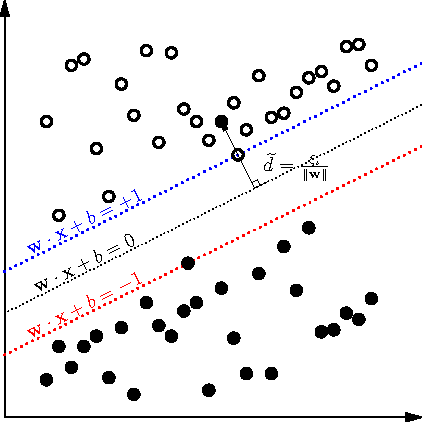
\includegraphics[scale=0.8]{fig/d2.pdf}
  \label{fig:d2}
\end{figure}

\noindent Introduce \emph{positive slack variables} $\ds\{\xi_i\}_{i=1}^m$ into the constraints
\begingroup
\addtolength{\jot}{-3pt}
\begin{align*}
  \vw\cdot\vx_i + b \geqslant +1 - \xi_i &\qquad\text{for }\,y_i=+1\\
  \vw\cdot\vx_i + b \leqslant -1 + \xi_i &\qquad\text{for }\,y_i=-1\\
  \xi_i\geqslant 0  &\qquad i=1,\,2,\,\ldots,\,m.
\end{align*}
\endgroup
The first two can be combined into
\begin{align*}
  1 - \xi_i - y_i\left(\vw\cdot\vx_i + b \right)\leqslant 0,\qquad i=1,\,2,\,\ldots,\,m
\end{align*}
If error occurs, $\xi_i > 1$; the objective function is changed to
\begin{align*}
  \text{minimize}\quad\frac{1}{2}\,\|\vw\|^2 + c\sum_{i=1}^m \xi_i
\end{align*}
where $c > 0$ controls the tolerance to errors on the training set. \\The Lagrangian with $2m$ multipliers $\lambda_i\geqslant 0$ and KKT conditions are
\begin{align}\label{f:lag1}
  \mathcal{L} = \frac{1}{2}\,\|\vw\|^2 + c\sum_{i=1}^m\xi_i + \sum_{i=1}^m\lambda_i\left\{1 - \xi_i - y_i\left(\vw\cdot\vx_i + b\right)\right\} - \sum_{i=1}^m\lambda_{m + i}\,\xi_i
\end{align}
\vspace{-8mm}
\begingroup
\addtolength{\jot}{-2pt}
\begin{equation}
\begin{aligned}\label{f:kkt1}
  &\frac{\partial\mathcal{L}}{\partial \vw} = 0 \ie \vw=\sum_{i=1}^m\lambda_i\,y_i\,\vx_i &\\
  &\frac{\partial\mathcal{L}}{\partial b} = 0 \ie \sum_{i=1}^m\lambda_iy_i=0 & \\
  &\frac{\partial\mathcal{L}}{\partial\xi_i} = 0 \ie c - \lambda_i-\lambda_{m + i} = 0, &i=1,\,2,\,\ldots,\,m\\
&\lambda_i\left\{1 - \xi_i - y_i\left(\vw\cdot\vx_i + b \right)\right\} = 0, &i=1,\,2,\,\ldots,\,m \\
  &1 - \xi_i - y_i\left(\vw\cdot\vx_i + b \right)\leqslant 0,\; &i=1,\,2,\,\ldots,\,m\\
  &\lambda_{m + i}\,\xi_i = 0,\quad\xi_i\geqslant 0, \quad & i=1,\,2,\,\ldots,\,m\\
  &\lambda_i\geqslant 0\qquad &i=1,\,2,\,\ldots,\,2m
\end{aligned}
\end{equation}
\endgroup
Substitute the KKT conditions (\ref{f:kkt1}) into $\mathcal{L}$ (\ref{f:lag1}), the dual Lagrangian 
\vspace{-1mm}
\begin{align*}
  \mathcal{L}_D=\sum_{i=1}^m\lambda_i-\frac{1}{2}\sum_{i=1}^m\sum_{j=1}^m\lambda_i\,\lambda_j\,y_i\,y_j\,\vx_i^\top\vx_j
\end{align*}
Now the problem becomes maximizing $\mathcal{L}_D$ subject to
\vspace{-1mm}
\begin{align*}
  0\leqslant\lambda_i\leqslant c\quad\text{and}\quad\sum_{i=1}^m\lambda_i y_i = 0.
\end{align*}

\newpage

\section*{Nonlinear SVM: Kernel Trick}
\begin{itemize}
  \item When the seperating boundary is not linear, map the data into another space $\mathcal{H}$ and perform classification there 
  \item Say the mapping function be $\Psi:\mathbb{R}^d\to\mathcal{H}$, the training algorithm now depends on $\Psi(\vx_i)\cdot\Psi(\vx_j)$ 
  \item If there were a ``kernel function'' $K$ such that $\ds K(\vx_i,\vx_j)=\Psi(\vx_i)\cdot\Psi(\vx_j)$, we don't need to know the exact form of $\Psi$
  \item \textbf{Mercer's condition}: $\ds K(\vx_i,\vx_j)=\Psi(\vx_i)\cdot\Psi(\vx_j) \ifff \\ \int K(\vx,{\bf y})g(\vx)g({\bf y})\,\text{d}\vx\,\text{d}{\bf y}\geqslant 0\quad\text{for square integrable functions }g$
  \item kernel examples:
    \begingroup
    \addtolength{\jot}{-2pt}
    \begin{align*}
      K(\vx_i,\vx_j)&=e^{-\frac{1}{2}(\vx_i-\vx_j)^\top\Sigma^{-1}(\vx_i-\vx_j)}\\
      K(\vx_i,\vx_j)&=\left(\vx_i^\top\vx_j + 1\right)^p \\
      K(\vx_i,\vx_j)&=\tanh\left(k\,\vx_i^\top\vx_j + \delta\right)
    \end{align*}
    \endgroup
\end{itemize}

\bibliographystyle{elsarticle-harv}
\bibliography{note09}

\end{document}
